\chapter{Álgebra}
%% recta numérica pequeña: \rectanum{xmin}{xmax}{dibujo}; marcas enteras con etiqueta en 0 y en los bordes que se pasen en #3
\newcommand{\rectanum}[3]{\begin{tikzpicture}[x=0.6cm,y=0.6cm,baseline=-3pt]
  \draw[gris] (#1-0.4,0) -- (#2+0.4,0);
  \foreach \k in {#1,...,#2} \draw[gris] (\k,-0.12) -- (\k,0.12);
  #3
\end{tikzpicture}}
\newcommand{\lleno}[1]{\fill[nar] (#1,0) circle (0.16); \node[below=1pt,font=\footnotesize] at (#1,-0.1) {$#1$};}
\newcommand{\vacio}[1]{\filldraw[draw=nar,fill=white,line width=1pt] (#1,0) circle (0.16); \node[below=1pt,font=\footnotesize] at (#1,-0.1) {$#1$};}
\newcommand{\tramo}[2]{\draw[nar,line width=2.4pt] (#1,0) -- (#2,0);}
\newcommand{\flechader}[2]{\draw[nar,line width=2.4pt,-{Stealth[length=7pt]}] (#1,0) -- (#2+0.5,0);}
\newcommand{\flechaizq}[2]{\draw[nar,line width=2.4pt,-{Stealth[length=7pt]}] (#2,0) -- (#1-0.5,0);}

%% =====================================================================
\section{Ecuaciones de primer grado}

\subsection{Qué es una ecuación}
Una \textbf{ecuación} es una igualdad con un número escondido, la \textbf{incógnita} (casi siempre $x$). El número que hace verdadera la igualdad es la \textbf{solución}: en $2x + 3 = 11$, la solución es $x = 4$, porque $2\cdot 4 + 3 = 11$. \textbf{Resolver} es encontrarla sin adivinar.

Es \textbf{de primer grado} (o lineal) porque la $x$ no tiene exponente: $5x - 1 = 9$ y $\dfrac{x}{3} + 2 = 7$ lo son; $x^2 = 9$ no lo es, y $3 + 4 = 7$ ni siquiera es ecuación, porque no tiene incógnita.

\subsection{La balanza: lo mismo a ambos lados}
\begin{minipage}[c]{0.56\linewidth}
Una ecuación es una balanza en equilibrio. En $2x + 3 = 11$ hay dos cajas de $x$ kg y una pesa de 3 kg contra una de 11 kg. Si sacamos 3 kg de cada lado, queda $2x = 8$; si repartimos cada lado en dos, queda $x = 4$.
\end{minipage}\hfill
\begin{minipage}[c]{0.4\linewidth}\centering
\begin{tikzpicture}[scale=0.8]
  \node[font=\bfseries] at (0,2.4) {$2x + 3 = 11$};
  \fill[nar] (0,0) -- (-0.55,-1.5) -- (0.55,-1.5) -- cycle;
  \fill[nard] (-0.9,-1.65) rectangle (0.9,-1.5);
  \draw[tinta,line width=2pt] (-2.9,0) -- (2.9,0);
  \draw[tinta,thick] (-1.75,0) -- (-1.75,0.45); \draw[tinta,thick] (1.75,0) -- (1.75,0.45);
  \draw[nard,line width=2pt] (-3.2,0.45) -- (-0.3,0.45); \draw[nard,line width=2pt] (0.3,0.45) -- (3.2,0.45);
  \foreach \p in {-3.1,-2.2} \draw[nar,thick,fill=hielo] (\p,0.5) rectangle ++(0.8,0.95) node[midway,font=\bfseries\itshape\color{nard}] {x};
  \draw[nard,fill=narc] (-1.3,0.5) rectangle ++(0.95,0.7) node[midway,font=\scriptsize\bfseries] {3 kg};
  \draw[nard,fill=narc] (1.0,0.5) rectangle ++(1.5,1.1) node[midway,font=\bfseries] {11 kg};
\end{tikzpicture}
\end{minipage}

\begin{clave}[La regla de oro] Puedes sumar, restar, multiplicar o dividir por un mismo número \textbf{a los dos lados} (sin dividir por 0). El atajo «pasar al otro lado» es lo mismo: lo que está \textbf{sumando} pasa \textbf{restando}, y lo que está \textbf{multiplicando} pasa \textbf{dividiendo}, y al revés.\end{clave}

\subsection{Despejar paso a paso}
\begin{clave}[Orden recomendado] 1. Quita los paréntesis. 2. Quita las fracciones. 3. Junta las $x$ en un lado y los números en el otro. 4. Divide por el número que acompaña a la $x$. 5. Comprueba en la ecuación del comienzo.\end{clave}
\begin{ejemplo} $7x - 4 = 3x + 12$: restando $3x$, $4x - 4 = 12$; sumando 4, $4x = 16$; dividiendo por 4, $x = 4$. Comprobación: $7\cdot 4 - 4 = 24$ y $3\cdot 4 + 12 = 24$.\end{ejemplo}
\begin{ojo}[El signo del número de la x] En $-3x = 12$ se divide por $-3$, con su signo: $x = \dfrac{12}{-3} = -4$.\end{ojo}

\subsection{Paréntesis y fracciones}
Un número delante de un paréntesis multiplica a \textbf{todo} lo de adentro, y un signo menos cambia el signo de \textbf{todo} lo de adentro:
\[ 4(x - 1) - (2x - 6) = 10 \;\Rightarrow\; 4x - 4 - 2x + 6 = 10 \;\Rightarrow\; 2x + 2 = 10 \;\Rightarrow\; x = 4. \]
Si hay fracciones, multiplica \textbf{todos} los términos, de los dos lados, por el mcm de los denominadores:
\[ \frac{x}{3} + \frac{x}{4} = 7 \;\overset{\cdot 12}{\Longrightarrow}\; 4x + 3x = 84 \;\Rightarrow\; x = 12. \]
\begin{ojo}[Los errores de siempre] $4(x - 1)$ no es $4x - 1$; $-(2x - 6)$ no es $-2x - 6$; y en $\dfrac{x}{2} + 1 = 4$, al multiplicar por 2 también se multiplican el 1 y el 4: $x + 2 = 8$. Si el numerador tiene dos términos, ponle paréntesis: $\dfrac{x + 2}{5}\cdot 10 = 2(x + 2)$.\end{ojo}
\gatotip[\gatogris]{Si una pregunta te muestra un procedimiento «con un error», rehaz cada paso tú mismo: el primero que no coincide es el culpable. Los siguientes solo arrastran el error.}

\subsection{Del enunciado a la ecuación}
Nombra lo que no sabes, escribe todo lo demás con esa letra, plantea y resuelve. «Es», «da» y «será» se traducen como $=$.

\begin{center}
\begin{tabular}{@{}ll@{\qquad}ll@{}}
\toprule
En palabras & Con $x$ & En palabras & Con $x$\\ \midrule
el doble de un número & $2x$ & 5 menos que el número & $x - 5$\\
la tercera parte & $\dfrac{x}{3}$ & el doble del número, más 3 & $2x + 3$\\
5 más que el número & $x + 5$ & el doble de la suma del número y 3 & $2(x + 3)$\\
tres consecutivos & $x,\ x+1,\ x+2$ & dos tipos que suman 20 & $x$ y $20 - x$\\ \bottomrule
\end{tabular}
\end{center}
\begin{ejemplo} La suma de tres consecutivos es 48: $x + (x+1) + (x+2) = 48$, así que $3x = 45$ y $x = 15$. Los números son 15, 16 y 17; si preguntan por el mayor, la respuesta es 17, no 15.\end{ejemplo}
\gatotip[\gatonegro]{Antes de marcar, relee qué te preguntan: muchas veces no es la $x$. Y si te quedas en blanco, reemplaza las alternativas: la correcta hace que los dos lados valgan lo mismo.}

\subsection{Sin solución o con infinitas}
A veces, al resolver, las $x$ se cancelan. Mira lo que queda:
\begin{center}
\begin{tabular}{@{}lll@{}}
\toprule
Al final queda & Significa & Ejemplo\\ \midrule
$x$ igual a un número & una sola solución & $4x = 0 \Rightarrow x = 0$\\
algo falso, como $1 = 6$ & ninguna solución & $2x + 1 = 2(x + 3)$\\
algo verdadero, como $6 = 6$ & infinitas soluciones & $3(x + 2) = 3x + 6$\\ \bottomrule
\end{tabular}
\end{center}
\begin{ojo}[x = 0 sí es una solución] $4x = 0$ tiene una solución, el cero. No la confundas con «no tiene solución».\end{ojo}

\begin{elejemplo}{PAES Invierno 2027, adaptada}
En una empresa que se dedica a la mantención y reparación de calefont trabajan Pedro, Joaquín, Rosario y Teresa como técnicos. En una semana de trabajo atendieron, entre los cuatro, un total de 79 clientes.

En dicha semana Pedro atendió 18 clientes, Joaquín atendió 8 clientes más que Rosario y Teresa atendió 9 clientes más que Joaquín.

¿Cuántos clientes atendió Rosario en esa semana de trabajo?
\alts{12}{18}{22}{36}
\solucion{Llamamos $x$ a los clientes de Rosario. Joaquín atendió $x + 8$; Teresa, 9 más que Joaquín (no que Rosario): $(x + 8) + 9 = x + 17$; Pedro, 18. La suma es el total:
\[ 18 + x + (x + 8) + (x + 17) = 79 \;\Rightarrow\; 3x + 43 = 79 \;\Rightarrow\; 3x = 36 \;\Rightarrow\; x = 12. \]
Comprobación: $18 + 12 + 20 + 29 = 79$. El 18 sale de olvidar sumar a Rosario; el 36 es $3x$, sin dividir por 3; con 22 el total sería 109.}{A}
\end{elejemplo}

%% =====================================================================
\section{Inecuaciones de primer grado}

\subsection{Desigualdades e inecuaciones}
Una \textbf{desigualdad} compara dos cantidades con $<$ (menor que), $>$ (mayor que), $\leq$ (menor o igual que) o $\geq$ (mayor o igual que). Una \textbf{inecuación} es una desigualdad con incógnita, como $x + 3 > 5$; resolverla es encontrar \textbf{todos} los valores que la cumplen. Aquí sirven todos los números mayores que 2, también los decimales: $x > 2$. Casi siempre hay infinitas soluciones.
\gatotip[\gatoatigrado]{La punta del símbolo apunta al más chico: en $2 < 5$ la punta mira al 2. La rayita de $\leq$ y $\geq$ significa «o igual».}

\subsection{Resolver, con una regla extra}
Se despeja igual que una ecuación: sumar o restar a ambos lados, o multiplicar y dividir por un positivo, no cambia el símbolo. Por ejemplo, $3x - 4 \leq 11 \Rightarrow 3x \leq 15 \Rightarrow x \leq 5$.
\begin{clave}[La regla clave] Si multiplicas o divides ambos lados por un número \textbf{negativo}, el símbolo se da vuelta: $<$ pasa a $>$ y $\leq$ pasa a $\geq$, y al revés.\end{clave}
\begin{ejemplo} De $2 < 5$, multiplicando por $-1$: $-2 > -5$. Y en $-2x + 1 > 7$: $-2x > 6$, y al dividir por $-2$ queda $x < -3$. Si no quieres dividir por un negativo, pasa la $x$ al otro lado: $1 - 7 > 2x$, o sea $-3 > x$, que es lo mismo.\end{ejemplo}
Por la misma regla, si $a < b$, entonces $a - 3 < b - 3$ y $\dfrac{a}{5} < \dfrac{b}{5}$, pero $-2a > -2b$.

\subsection{El conjunto solución: intervalos y recta numérica}
La solución se escribe como desigualdad, como intervalo o en la recta. \textbf{Punto lleno} y corchete que abraza al número ($[1$, $3]$): el número está incluido ($\leq$, $\geq$). \textbf{Punto vacío} y corchete hacia afuera ($]1$, $3[$): no está incluido ($<$, $>$).
\begin{center}
\renewcommand{\arraystretch}{1.6}
\begin{tabular}{@{}lll@{}}
\toprule
Desigualdad & Intervalo & Recta numérica\\ \midrule
$x \geq -1$ & $[-1, +\infty[$ & \rectanum{-2}{3}{\flechader{-1}{3}\lleno{-1}}\\
$x < 2$ & $\mathopen{]}-\infty, 2\mathclose{[}$ & \rectanum{-2}{3}{\flechaizq{-2}{2}\vacio{2}}\\
$1 \leq x < 3$ & $[1, 3[$ & \rectanum{-1}{4}{\tramo{1}{3}\lleno{1}\vacio{3}}\\ \bottomrule
\end{tabular}
\end{center}
\begin{ojo}[El infinito no se alcanza] Al lado de $+\infty$ o $-\infty$ el corchete va siempre abierto: $[2, +\infty[$, nunca $[2, +\infty]$.\end{ojo}

\subsection{Traducir el enunciado}
\begin{center}
\begin{tabular}{@{}p{0.47\linewidth}cl@{}}
\toprule
Frase & Símbolo & Ejemplo\\ \midrule
a lo menos, como mínimo, al menos, no menos de & $\geq$ & nota a lo menos 4,0: $x \geq 4$\\
como máximo, a lo más, no supera, no puede ser mayor que & $\leq$ & dosis no mayor que 2.000 mg\\
más de, supera, mayor que & $>$ & más de 18 años: $e > 18$\\
menos de, menor que & $<$ & menos de 5 °C: $t < 5$\\ \bottomrule
\end{tabular}
\end{center}
«A lo menos 5» incluye el 5; «más de 5» no. Esa diferencia decide el punto lleno o vacío, y muchas veces la respuesta.

\subsection{Respuestas enteras, notas y planes}
\begin{ejemplo}[Como máximo] Una camioneta carga a lo más 1.000 kg; el conductor pesa 70 kg y los sacos, 40 kg: $70 + 40x \leq 1.000$, o sea $x \leq 23{,}25$. Los sacos son enteros: como máximo 23.\end{ejemplo}
\begin{ojo}[Redondea según la pregunta] Con «como máximo» se redondea hacia abajo (23,9 da 23); con «como mínimo», hacia arriba ($x \geq 7{,}2$ cajas da 8).\end{ojo}
\begin{ejemplo}[Inecuación doble] En $-3 < 2x + 1 \leq 7$ se opera en las tres partes: $-4 < 2x \leq 6$, así que $-2 < x \leq 3$. El $-2$ queda fuera y el 3 entra: los enteros son $-1, 0, 1, 2, 3$.\par\smallskip
\centering\rectanum{-3}{4}{\tramo{-2}{3}\vacio{-2}\lleno{3}}\end{ejemplo}
\begin{ejemplo}[Nota mínima] Con 4,0; 5,2 y 6,0, para un promedio de a lo menos 5,5: $\dfrac{15{,}2 + x}{4} \geq 5{,}5 \Rightarrow 15{,}2 + x \geq 22 \Rightarrow x \geq 6{,}8$. La mínima es justo el borde.\end{ejemplo}
\begin{ejemplo}[Comparar planes] Plan A: \peso 10.000 más \peso 40 por minuto; plan B: \peso 16.000 más \peso 25. B es más barato si $16.000 + 25x < 10.000 + 40x$, o sea $x > 400$. En 400 minutos cuestan lo mismo (el empate no cuenta): conviene desde 401.\end{ejemplo}
\gatotip[\gatolila]{Comprueba siempre con dos números: el borde, que solo cumple si hay «o igual», y uno de afuera, que no debe cumplir.}

\begin{elejemplo}{PAES Invierno 2026, adaptada}
La dosis de un medicamento solo es efectiva si se suministran como mínimo 25 mg por kilogramo de peso del paciente, una vez al día, pero la dosis diaria no puede ser mayor que 2.000 mg.

¿Cuántos kilogramos, como máximo, debe tener un paciente para que este medicamento sea efectivo y no supere la dosis diaria?
\alts{25 kg}{55 kg}{80 kg}{105 kg}
\solucion{Si el paciente pesa $x$ kg, la dosis más chica que le sirve es $25x$ mg. «No puede ser mayor que 2.000» es $\leq$: $25x \leq 2.000$. Dividiendo por 25, que es positivo, $x \leq 80$. El máximo es el borde, 80 kg, porque $\leq$ lo incluye. Comprobación: con 80 kg la dosis es justo 2.000 mg; con 81 kg ya son 2.025 mg. El 25 confunde la dosis con el peso, 55 sirve pero no es el máximo y con 105 kg se pasa del tope.}{C}
\end{elejemplo}

%% =====================================================================
\section{Operatoria con expresiones algebraicas}

\subsection{Las piezas de una expresión}
Una \textbf{expresión algebraica} mezcla números y letras con operaciones. En $5x^2y - 3x + 7$ hay tres \textbf{términos}; en cada uno, el \textbf{coeficiente} es el número con su signo ($5$, $-3$) y el \textbf{factor literal} son las letras con sus exponentes ($x^2y$). Si no se ve el coeficiente, es 1: $x = 1\cdot x$ y $-x = -1\cdot x$. Con un término es un monomio; con dos, binomio; con tres, trinomio; en general, polinomio.
\begin{clave}[Términos semejantes] Tienen exactamente el mismo factor literal: $4x$ y $-9x$ sí; $3ab$ y $7ba$ sí; $2x^2$ y $2x$ no; $5xy$ y $5x$ no. Solo esos se pueden juntar.\end{clave}

\subsection{Reducir}
Se suman o restan los coeficientes y el factor literal se copia igual: $7x + 3y - 2x + 5y - y = 5x + 7y$. Con paréntesis, un menos delante cambia el signo de \textbf{todo} lo de adentro y un más lo deja igual:
\[ 3a - (2a - 5b) + (a + b) = 3a - 2a + 5b + a + b = 2a + 6b. \]
\begin{ojo}[Los exponentes no se suman al reducir] $x^2 + x^2 = 2x^2$, no $x^4$; y $3x + 2y$ se queda así, no es $5xy$.\end{ojo}
\gatotip[\gatoblanco]{3 manzanas más 2 manzanas son 5 manzanas, pero 3 manzanas más 2 peras no son 5 «manzaperas». Lo mismo pasa con $3x + 2y$.}

\subsection{Valorizar}
Valorizar es reemplazar cada letra por su número y calcular, en este orden: paréntesis, potencias, multiplicaciones y divisiones, sumas y restas.
\begin{ejemplo} Con $a = -2$ y $b = 3$: $3a^2 - 2ab + b = 3(-2)^2 - 2(-2)(3) + 3 = 12 + 12 + 3 = 27$.\end{ejemplo}
\begin{ojo}[El paréntesis salva el signo] $(-2)^2 = 4$, pero $-2^2 = -4$. Reemplaza los negativos siempre entre paréntesis. Con fracciones, eleva primero: si $x = \frac{1}{2}$, $4x^2 = 4\cdot\frac{1}{4} = 1$; y dividir por $\frac{1}{2}$ es multiplicar por 2.\end{ojo}

\subsection{Multiplicar monomios y polinomios}
\begin{minipage}[c]{0.6\linewidth}
\textbf{Monomio por monomio:} se multiplican los coeficientes y, en cada letra, se \textbf{suman} los exponentes: $(2x^3y)(-5xy^2) = -10x^4y^3$.

\textbf{Monomio por polinomio:} el monomio multiplica a \textbf{cada} término: $3a(2a + 4) = 6a^2 + 12a$. En la figura, el rectángulo se parte en dos y sus áreas suman el total.

\textbf{Polinomio por polinomio:} cada término del primero por cada término del segundo, y se reduce: $(x + 3)(2x - 5) = 2x^2 - 5x + 6x - 15 = 2x^2 + x - 15$.
\end{minipage}\hfill
\begin{minipage}[c]{0.36\linewidth}\centering
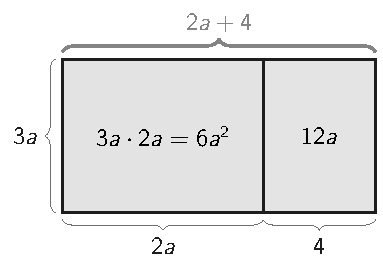
\includegraphics[width=0.95\linewidth]{expr_distributiva}
\end{minipage}
\begin{ojo}[Signos] $(+)(+) = +$, $(-)(-) = +$, $(+)(-) = -$. Así, $-2x(x - 4) = -2x^2 + 8x$. Y al multiplicar se suman exponentes: $x^2\cdot x^3 = x^5$, no $x^6$.\end{ojo}

\subsection{Del lenguaje natural al algebraico}
Lee la frase de afuera hacia adentro: la última operación que se nombra es la que manda. Si la edad de Pedro es $m$, «su edad hace $n$ años disminuida en 3» es $m - n - 3$; «el doble de la suma de un número y 5» es $2(x + 5)$, pero «el doble de un número, más 5» es $2x + 5$.
\begin{center}
\begin{tabular}{@{}ll@{\qquad}ll@{}}
\toprule
En palabras & Expresión & En palabras & Expresión\\ \midrule
el cuadrado de la suma de $a$ y $b$ & $(a + b)^2$ & el triple de la diferencia entre $x$ y 2 & $3(x - 2)$\\
la suma de los cuadrados & $a^2 + b^2$ & dos consecutivos & $n$ y $n + 1$\\
4 menos que $x$ & $x - 4$ & un número par & $2n$\\ \bottomrule
\end{tabular}
\end{center}

\subsection{Perímetros y áreas con expresiones}
Si un rectángulo mide $(2x + 3)$ por $(x - 1)$, su \textbf{perímetro} es $2(2x + 3) + 2(x - 1) = 6x + 4$ y su \textbf{área} es $(2x + 3)(x - 1) = 2x^2 + x - 3$. Con $x = 4$ mide 11 por 3: perímetro 28 y área 33, igual que con las expresiones.
\begin{ojo}[No confundas] El perímetro suma lados (no aparece $x^2$); el área los multiplica. Y para lo que sobra se resta \textbf{todo}, con paréntesis: $(10x + 8) - (6x + 4) = 4x + 4$.\end{ojo}
\gatotip[\gatonaranjo]{¿Dudas entre alternativas? Reemplaza la letra por un número sencillo, como 2, en el enunciado y en cada alternativa: la correcta da lo mismo.}

\begin{elejemplo}{PAES Regular 2026}
Una pista de baile de forma rectangular tiene dimensiones de $(3x + 4)$ metros de largo y $(2x - 9)$ metros de ancho. Se cuenta con $(20x + 20)$ metros de una cinta luminosa para demarcar el borde de la pista de baile.
\begin{center}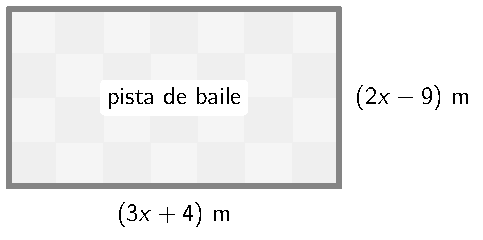
\includegraphics[width=5.2cm]{expr_pista}\end{center}
¿Cuántos metros de cinta luminosa sobran luego de demarcar el borde de la pista?
\alts{$(10x + 30)$ metros}{$(10x + 10)$ metros}{$(15x + 15)$ metros}{$(15x + 25)$ metros}
\solucion{Demarcar el borde es recorrer el perímetro: $2(3x + 4) + 2(2x - 9) = 6x + 8 + 4x - 18 = 10x - 10$. Lo que sobra es la cinta menos todo el perímetro:
\[ (20x + 20) - (10x - 10) = 20x + 20 - 10x + 10 = 10x + 30. \]
Comprobación con $x = 10$: la pista mide 34 m por 11 m, su perímetro es 90 m, la cinta mide 220 m y sobran 130 m $= 10\cdot 10 + 30$. $(10x + 10)$ cambia solo el primer signo del paréntesis; $(15x + 25)$ y $(15x + 15)$ restan medio perímetro.}{A}
\end{elejemplo}

%% =====================================================================
\section{Productos notables}

\subsection{Qué es un producto notable}
Son multiplicaciones tan frecuentes que conviene saber su resultado de memoria. Todas salen de multiplicar término a término, pero reconocer el molde ahorra tiempo y errores de signo.
\begin{clave}[Los cuatro moldes]
\[ (a + b)^2 = a^2 + 2ab + b^2 \qquad (a - b)^2 = a^2 - 2ab + b^2 \]
\[ (a + b)(a - b) = a^2 - b^2 \qquad (x + p)(x + q) = x^2 + (p + q)x + pq \]
Las letras son moldes: en $(2x + 5)^2$, $a = 2x$ y $b = 5$.\end{clave}

\subsection{Cuadrado de binomio}
\begin{minipage}[c]{0.62\linewidth}
En palabras: \textbf{el cuadrado del primero, más (o menos) el doble del primero por el segundo, más el cuadrado del segundo}. El dibujo lo muestra: el cuadrado de lado $a + b$ se parte en $a^2$, $b^2$ y \textbf{dos} rectángulos $ab$.
\[ (x + 5)^2 = x^2 + 10x + 25 \qquad (2x + 3)^2 = 4x^2 + 12x + 9 \]
\[ (x - 4)^2 = x^2 - 8x + 16 \qquad (3x - 2y)^2 = 9x^2 - 12xy + 4y^2 \]
En la resta, el término del medio es negativo y el último \textbf{siempre es positivo}. Además, $(a - b)^2 = (b - a)^2$.
\end{minipage}\hfill
\begin{minipage}[c]{0.34\linewidth}\centering
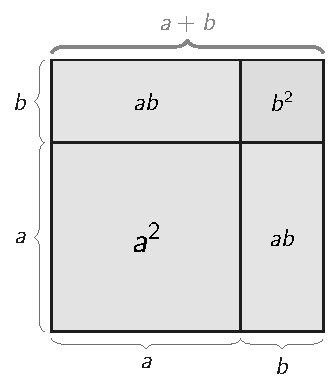
\includegraphics[width=0.85\linewidth]{expr_cuadrado_binomio}
\end{minipage}
\begin{ojo}[El error más común de la PAES] $(a + b)^2 \ne a^2 + b^2$: faltan los dos rectángulos. Con números, $(3 + 4)^2 = 49$, pero $3^2 + 4^2 = 25$. Revisa los tres términos: $(x - 4)^2$ no es $x^2 - 16$, ni $x^2 - 8x - 16$, ni $x^2 - 4x + 16$.\end{ojo}
\gatotip[\gatoatigrado]{Cálculo mental: $21^2 = (20 + 1)^2 = 400 + 40 + 1 = 441$ y $99^2 = (100 - 1)^2 = 10.000 - 200 + 1 = 9801$.}

\subsection{Suma por diferencia}
\begin{minipage}[c]{0.5\linewidth}
Al multiplicar, los términos del medio se cancelan: $(a + b)(a - b) = a^2 - ab + ab - b^2 = a^2 - b^2$. En el dibujo, a un cuadrado de lado $a$ se le quita uno de lado $b$ y lo que queda se reordena en un rectángulo de lados $a + b$ y $a - b$.

$(x + 7)(x - 7) = x^2 - 49$, \quad $(3x + 2y)(3x - 2y) = 9x^2 - 4y^2$ \quad y \quad $103\cdot 97 = 100^2 - 3^2 = 9991$.
\end{minipage}\hfill
\begin{minipage}[c]{0.46\linewidth}\centering
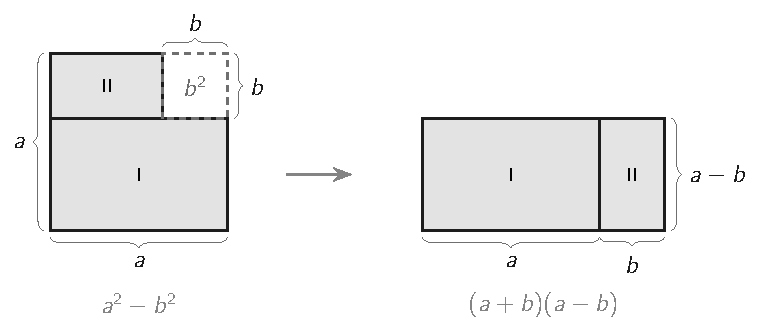
\includegraphics[width=\linewidth]{expr_suma_diferencia}
\end{minipage}
\begin{ojo}[Mismos términos, un signo distinto] $(x + 3)(x - 2)$ no es suma por diferencia.\end{ojo}

\subsection{Binomios con término común}
\begin{minipage}[c]{0.62\linewidth}
En $(x + p)(x + q)$ el resultado es $x^2$, más \textbf{la suma} de los números por $x$, más \textbf{su producto}. En el dibujo, $(x + 4)(x + 3) = x^2 + 7x + 12$.
\[ (x - 5)(x + 2) = x^2 - 3x - 10 \qquad (x - 2)(x - 6) = x^2 - 8x + 12 \]
Si $p = q$ es un cuadrado de binomio; si $q = -p$, una suma por diferencia.
\end{minipage}\hfill
\begin{minipage}[c]{0.34\linewidth}\centering
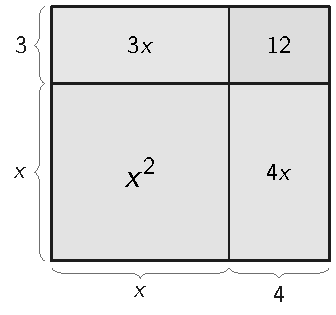
\includegraphics[width=0.8\linewidth]{expr_binomios_comun}
\end{minipage}

\subsection{Combinar productos notables}
Desarrolla cada producto por separado y \textbf{resta con paréntesis}:
\[ (x + 3)^2 - (x + 3)(x - 3) = (x^2 + 6x + 9) - (x^2 - 9) = x^2 + 6x + 9 - x^2 + 9 = 6x + 18. \]
\begin{ejemplo}[Usar datos sin despejar] Si $a + b = 7$ y $ab = 10$: $a^2 + b^2 = (a + b)^2 - 2ab = 49 - 20 = 29$, sin saber cuánto valen $a$ y $b$.\end{ejemplo}
\begin{ojo}[Errores típicos] $(2x)^2 = 4x^2$, no $2x^2$. $(x + 5)^2$ lleva $10x$, no $5x$. $(x + 4)(x - 4) = x^2 - 16$, no $x^2 + 16$. Y al restar $x^2 - 9$, el $-9$ se vuelve $+9$.\end{ojo}
\gatotip[\gatogris]{Comprueba con $x = 1$: la expresión original y tu resultado deben dar el mismo número.}

\begin{elejemplo}{PAES Invierno 2026}
¿Cuál de las siguientes expresiones es igual a $(2x - 3)^2 - (2x - 3)(2x + 3)$?
\alts{$18$}{$0$}{$-6x + 18$}{$-12x + 18$}
\solucion{Cuadrado de binomio con $a = 2x$ y $b = 3$: $(2x - 3)^2 = 4x^2 - 12x + 9$. Suma por diferencia: $(2x - 3)(2x + 3) = 4x^2 - 9$. Restando con paréntesis:
\[ (4x^2 - 12x + 9) - (4x^2 - 9) = 4x^2 - 12x + 9 - 4x^2 + 9 = -12x + 18. \]
Comprobación con $x = 1$: $1 - (-5) = 6$ y $-12 + 18 = 6$. El 18 olvida el término del medio, el 0 cree que los dos productos son iguales y $-6x + 18$ olvida el 2 del doble producto.}{D}
\end{elejemplo}

%% =====================================================================
\section{Factorización}

\subsection{Factorizar es deshacer la multiplicación}
\textbf{Factorizar} es escribir una suma como una multiplicación: el camino inverso de desarrollar. $3a(2a + 4) \to 6a^2 + 12a$ es desarrollar; $6a^2 + 12a \to 6a(a + 2)$ es factorizar. Con números ya lo haces: $12 + 20 = 4(3 + 5)$. Siempre se puede comprobar multiplicando.
\begin{ojo}[Factoriza completo] $3a(2a + 4)$ es igual a $6a^2 + 12a$, pero en el paréntesis queda un 2 común. La factorización completa saca el \textbf{mayor} factor común: $6a(a + 2)$.\end{ojo}

\subsection{Factor común}
\begin{clave}[Cómo encontrarlo] Números: su MCD. Letras: cada letra que está en \textbf{todos} los términos, con su \textbf{menor} exponente. Después divide cada término por el factor común.\end{clave}
\begin{ejemplo} $12x^3 - 18x^2$: MCD 6 y letra $x^2$, así que $12x^3 - 18x^2 = 6x^2(2x - 3)$. Si un término «desaparece» queda 1: $5x + 5 = 5(x + 1)$. El factor común puede ser un paréntesis: $x(a + b) + 3(a + b) = (a + b)(x + 3)$.\end{ejemplo}
\gatotip[\gatonegro]{Cálculo mental: $37\cdot 13 + 37\cdot 87 = 37(13 + 87) = 3700$. El 37 sale una sola vez.}

\subsection{Diferencia de cuadrados}
\begin{clave} \[ a^2 - b^2 = (a + b)(a - b) \] Dos cuadrados separados por un menos. Se usan sus \textbf{raíces}.\end{clave}
\begin{ejemplo} $x^2 - 49 = (x + 7)(x - 7)$; $9x^2 - 16y^2 = (3x + 4y)(3x - 4y)$; $2x^2 - 50 = 2(x^2 - 25) = 2(x + 5)(x - 5)$; $51^2 - 49^2 = 100\cdot 2 = 200$.\end{ejemplo}
\begin{ojo}[La suma de cuadrados no se factoriza así] $x^2 + 9$ no es $(x + 3)(x - 3)$, que da $x^2 - 9$, ni $(x + 3)^2$, que da $x^2 + 6x + 9$.\end{ojo}

\subsection{Trinomio cuadrado perfecto}
\begin{clave} \[ a^2 + 2ab + b^2 = (a + b)^2 \qquad a^2 - 2ab + b^2 = (a - b)^2 \] Los extremos son cuadrados positivos; saca sus raíces; el término del medio debe ser el \textbf{doble} de su producto, y su signo dice si es suma o resta.\end{clave}
\begin{ejemplo} $x^2 + 10x + 25$: raíces $x$ y 5, y $2\cdot x\cdot 5 = 10x$: es $(x + 5)^2$. $4x^2 - 12x + 9 = (2x - 3)^2$. En cambio, $x^2 + 6x + 25$ no es cuadrado perfecto: el medio debería ser $10x$.\end{ejemplo}

\subsection{Trinomio x² + bx + c}
\begin{minipage}[c]{0.64\linewidth}
\[ x^2 + bx + c = (x + p)(x + q) \quad\text{con}\quad p + q = b,\ \ pq = c \]
Busca \textbf{dos números que multiplicados den $c$ y sumados den $b$}. En $x^2 + 7x + 12$ son 3 y 4: $(x + 3)(x + 4)$, el rectángulo del dibujo.
\begin{clave}[Regla de signos] Si $c$ es positivo, los dos números tienen el signo de $b$: $x^2 - 9x + 20 = (x - 4)(x - 5)$. Si $c$ es negativo, tienen signos distintos: $x^2 - 2x - 15 = (x - 5)(x + 3)$.\end{clave}
\end{minipage}\hfill
\begin{minipage}[c]{0.32\linewidth}\centering
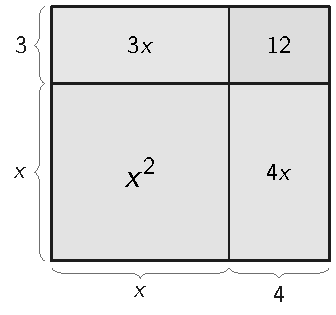
\includegraphics[width=0.85\linewidth]{expr_binomios_comun}
\end{minipage}

\subsection{Simplificar fracciones algebraicas}
Solo se tachan \textbf{factores} (cosas que multiplican), nunca sumandos. Por eso primero se factoriza:
\[ \frac{x^2 - 9}{x + 3} = \frac{(x + 3)(x - 3)}{x + 3} = x - 3 \ \ (x \ne -3), \qquad \frac{x^2 + 5x}{x^2 - 25} = \frac{x(x + 5)}{(x + 5)(x - 5)} = \frac{x}{x - 5}. \]
El valor que anula el denominador original queda excluido también después de simplificar.
\begin{ojo}[Así no] $\dfrac{x + 6}{x + 2} \ne \dfrac{6}{2}$. Con $x = 2$ vale $\dfrac{8}{4} = 2$, no 3.\end{ojo}

\subsection{Qué factorización uso}
\begin{center}
\small\begin{tabular}{@{}lll@{}}
\toprule
Mira esto & Usa & Ejemplo\\ \midrule
algo se repite en todos los términos & factor común (siempre primero) & $4x^2 + 6x = 2x(2x + 3)$\\
dos cuadrados con un menos & diferencia de cuadrados & $x^2 - 36 = (x + 6)(x - 6)$\\
extremos cuadrados y medio $2ab$ & trinomio cuadrado perfecto & $x^2 - 8x + 16 = (x - 4)^2$\\
$x^2 + bx + c$ & producto $c$, suma $b$ & $x^2 + x - 12 = (x + 4)(x - 3)$\\ \bottomrule
\end{tabular}
\end{center}
Después revisa si algún paréntesis se puede factorizar de nuevo: $3x^2 - 12 = 3(x + 2)(x - 2)$ y $2x^3 - 8x^2 + 8x = 2x(x - 2)^2$. Si un producto vale 0, algún factor vale 0: $(p - 3)^2 - 36 = (p + 3)(p - 9) = 0$ da $p = -3$ o $p = 9$.
\gatotip[\gatolila]{Con un área y un lado, factoriza el área: si mide $x^2 + 7x + 12$ y un lado es $x + 3$, el otro es $x + 4$. Y descarta las medidas negativas.}

\begin{elejemplo}{PAES Regular 2026, adaptada}
Una persona realiza el siguiente procedimiento para factorizar $12x^2 + 20x$, cometiendo un error.

Paso 1: escribe cada término como un producto, obteniendo $4\cdot 3\cdot x\cdot x + 4\cdot 5\cdot x$.\\
Paso 2: descompone cada número en factores primos, obteniendo $2\cdot 2\cdot 3\cdot x\cdot x + 2\cdot 2\cdot 5\cdot x$.\\
Paso 3: escribe las potencias correspondientes, obteniendo $2^2\cdot 3\cdot x^2 + 2^2\cdot 5\cdot x$.\\
Paso 4: factoriza la suma, obteniendo $2^4x(3x + 5)$.

¿En cuál de los pasos la persona cometió el error?
\alts{En el Paso 1}{En el Paso 2}{En el Paso 3}{En el Paso 4}
\solucion{Los Pasos 1, 2 y 3 solo reescriben los números: cada expresión sigue siendo igual a $12x^2 + 20x$. En el Paso 4, el factor común es lo que se repite en los dos términos, $2^2$ y $x$, o sea $4x$; la persona sumó los exponentes de los dos $2^2$ y escribió $2^4 = 16$. Lo que se repite se saca \textbf{una vez}. Lo correcto es $12x^2 + 20x = 4x(3x + 5)$; en cambio, $2^4x(3x + 5) = 48x^2 + 80x$, el cuádruple de lo pedido.}{D}
\end{elejemplo}

%% =====================================================================
\section{Proporcionalidad directa}

\subsection{Razón y proporción}
Una \textbf{razón} compara dos cantidades dividiéndolas: 12 niñas y 18 niños están en la razón $12 : 18 = \frac{12}{18} = 2 : 3$, es decir, por cada 2 niñas hay 3 niños. Una \textbf{proporción} es una igualdad de razones, como $\frac{2}{3} = \frac{8}{12}$.
\begin{clave}[Propiedad fundamental] $\dfrac{a}{b} = \dfrac{c}{d}$ es lo mismo que $a\cdot d = b\cdot c$ (producto cruzado). Con ella se despeja el término que falta: $\dfrac{x}{15} = \dfrac{2}{3} \Rightarrow 3x = 30 \Rightarrow x = 10$.\end{clave}
\begin{ojo}[El orden importa] Cuando dice \textbf{respectivamente}, el primer número va con lo primero que se nombra. Y si la razón es $2 : 3$, el grupo tiene $2 + 3 = 5$ partes: las niñas son $\frac{2}{5}$ del curso, no $\frac{2}{3}$.\end{ojo}

\subsection{Qué es la proporcionalidad directa}
Dos cantidades son \textbf{directamente proporcionales} si, cuando una se multiplica por un número, la otra se multiplica por el \textbf{mismo} número: el doble con el doble, la mitad con la mitad. El cociente es constante:
\begin{clave} \[ \frac{y}{x} = k \qquad\Longleftrightarrow\qquad y = k\cdot x \] La constante $k$ es lo que vale $y$ cuando $x = 1$: el precio de \textbf{un} cuaderno, lo que se paga por \textbf{un} minuto. Se llama valor unitario.\end{clave}
\begin{center}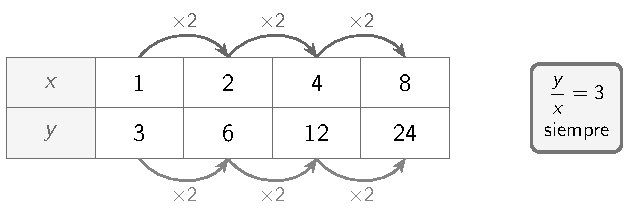
\includegraphics[width=8.2cm]{prop_tabla_directa}\end{center}
\textbf{En una tabla}, divide $y$ por $x$ en cada columna: con $x$: 2, 5, 8 e $y$: 6, 15, 24 siempre da 3, así que es directa. Con $x$: 1, 2, 3 e $y$: 5, 7, 9 da 5; 3,5 y 3: no lo es (es $y = 2x + 3$).
\begin{ojo}[Que las dos crezcan no basta] Al pasar de $x = 1$ a $x = 2$, $y$ debe duplicarse. Además, si $x = 0$, entonces $y = 0$: con un cobro fijo (la bajada de bandera de un taxi) ya no es proporcional.\end{ojo}

\subsection{El gráfico: una recta que pasa por el origen}
\begin{minipage}[c]{0.5\linewidth}
Los puntos $(x, y)$ de $y = kx$ quedan sobre una recta que pasa por $(0, 0)$. Para leer $k$, toma un punto distinto del origen y divide su altura por su $x$: con $(4, 12)$, $k = 3$. Cada vez que avanzas 1, la recta sube $k$: $k$ es la pendiente.

En cambio, $y = 3x + 2$ también es una recta, pero corta el eje $Y$ en 2: no es proporcionalidad directa.
\end{minipage}\hfill
\begin{minipage}[c]{0.46\linewidth}\centering
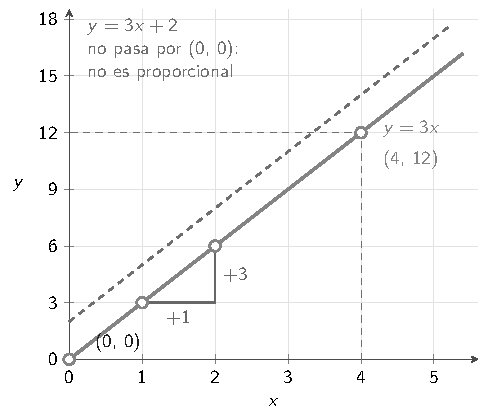
\includegraphics[width=0.92\linewidth]{prop_graf_directa}
\end{minipage}

\subsection{La regla de tres directa}
\begin{ejemplo} 4 kg de paltas cuestan \peso 7200; ¿cuánto cuestan 6 kg? \textbf{Valor unitario:} 1 kg cuesta $\frac{7200}{4} = 1800$, y 6 kg, $6\cdot 1800 = 10.800$. \textbf{Proporción:} $\frac{4}{7200} = \frac{6}{x}$, así que $4x = 43.200$ y $x = 10.800$.\end{ejemplo}
\begin{ojo}[Revisa el sentido] Kilos arriba y pesos abajo en las dos razones. Si te da que 6 kg cuestan menos que 4 kg, armaste mal la proporción. Y si una cantidad aumenta en 100, la otra no aumenta en 100: aumenta en la misma \textbf{proporción}.\end{ojo}
\gatotip[\gatoblanco]{Las escalas de mapas son proporción directa: si 1 cm equivale a 50 m, 7 cm son $7\cdot 50 = 350$ m. Calcula primero lo que vale 1 cm.}

\subsection{Repartos proporcionales}
\begin{clave}[Repartir en la razón $a : b$] Cuenta las partes, $a + b$; divide el total por ese número para obtener una parte, y multiplica por las partes de cada uno.\end{clave}
\begin{ejemplo} \peso 60.000 en la razón $2 : 3$: son 5 partes de 12.000; Ana recibe 24.000 y Beto 36.000. Si se reparte según lo que aportó cada uno (\peso 3000 y \peso 2000), la razón es $3 : 2$.\end{ejemplo}
\begin{ojo}[No dividas por 2] Repartir en la razón $2 : 3$ no es repartir por mitades, ni dividir por 2 y por 3: se divide por el total de partes, 5.\end{ojo}

\begin{elejemplo}{PAES Invierno 2026, adaptada}
Javier y David compraron una bolsa de 24 dulces a un precio total de \peso 2100, tal que Javier aportó \peso 1400 y David aportó el resto del dinero.

Ellos deciden vender cada dulce a \peso 200 y repartirse el dinero obtenido de forma proporcional a lo que aportó cada uno en la compra.

¿Cuánto dinero recibirá Javier luego de vender todos los dulces?
\alts{\peso 1600}{\peso 2400}{\peso 2700}{\peso 3200}
\solucion{La venta da $24\cdot 200 = 4800$ pesos. David aportó $2100 - 1400 = 700$, así que los aportes están en la razón $1400 : 700 = 2 : 1$. Son $2 + 1 = 3$ partes de $\frac{4800}{3} = 1600$, y Javier recibe 2 partes: $3200$ pesos. Comprobación: David recibe 1600 y $3200 + 1600 = 4800$. \peso 1600 es lo de David, \peso 2400 reparte por mitades y \peso 2700 es la ganancia total.}{D}
\end{elejemplo}

%% =====================================================================
\section{Proporcionalidad inversa}

\subsection{Qué es la proporcionalidad inversa}
Dos cantidades son \textbf{inversamente proporcionales} si, cuando una se multiplica por un número, la otra se \textbf{divide} por ese mismo número: si una se duplica, la otra se reduce a la mitad. Al repartir 24 caramelos entre 1, 2, 4 u 8 niños tocan 24, 12, 6 o 3: el producto siempre es 24.
\begin{clave} \[ x\cdot y = k \qquad\Longleftrightarrow\qquad y = \frac{k}{x} \] La constante $k$ es el total: lo que se reparte, la distancia del viaje, el trabajo de la obra.\end{clave}
\begin{center}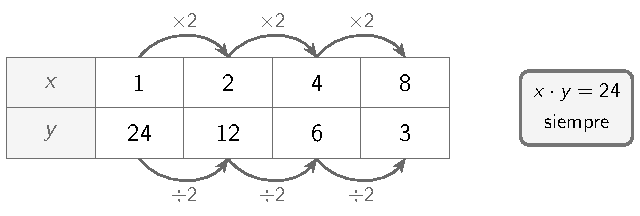
\includegraphics[width=8.2cm]{prop_tabla_inversa}\end{center}

\subsection{Cómo reconocerla}
En una tabla, \textbf{multiplica} $x$ por $y$ en cada columna. A 60 km/h se tarda 4 h, a 80 km/h 3 h y a 120 km/h 2 h: el producto es siempre 240 (la distancia), así que es inversa. Con $x$: 1, 2, 3 e $y$: 10, 8, 6 los productos son 10, 16 y 18: no lo es.
\begin{center}
\begin{tabular}{@{}lll@{}}
\toprule
 & Directa & Inversa\\ \midrule
lo constante & $\dfrac{y}{x} = k$ & $x\cdot y = k$\\[6pt]
fórmula & $y = kx$ & $y = \dfrac{k}{x}$\\[6pt]
si $x$ se duplica & $y$ se duplica & $y$ se divide por 2\\
gráfico & recta por el origen & hipérbola\\ \bottomrule
\end{tabular}
\end{center}
\begin{ojo}[Que una baje cuando la otra sube no basta] En $y = 10 - x$, $y$ baja, pero $1\cdot 9 = 9$ y $2\cdot 8 = 16$. Revisa \textbf{todas} las columnas.\end{ojo}

\subsection{El gráfico: una hipérbola}
\begin{minipage}[c]{0.5\linewidth}
Los puntos de $y = \frac{24}{x}$ forman una curva llamada \textbf{hipérbola}: cuando $x$ crece, $y$ baja, primero rápido y después cada vez más lento. Se acerca a los ejes pero \textbf{nunca los toca}, porque $x$ e $y$ no pueden valer 0.

Desde el origen hasta cada punto se forma un rectángulo de área $x\cdot y = 24$: todos tienen la misma área.
\end{minipage}\hfill
\begin{minipage}[c]{0.46\linewidth}\centering
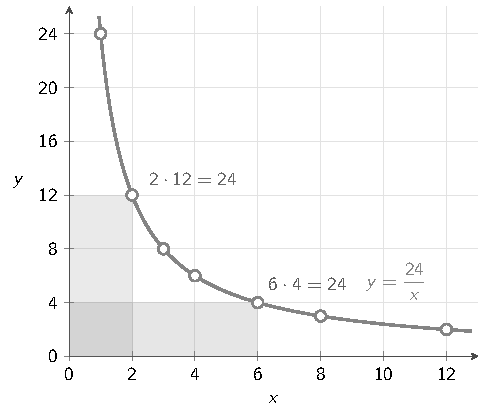
\includegraphics[width=0.92\linewidth]{prop_graf_inversa}
\end{minipage}

\subsection{Trabajadores, rapidez, raciones y llaves}
\begin{clave}[Método] 1. ¿Más de una da menos de la otra? 2. Calcula $k = x\cdot y$, el total. 3. Divide $k$ por la nueva cantidad. 4. Revisa el sentido.\end{clave}
\begin{ejemplo}[Trabajadores] 6 obreros tardan 10 días: la obra son $6\cdot 10 = 60$ «días de un obrero». Con 4 obreros: $\frac{60}{4} = 15$ días. Con proporción, sin dar vuelta nada: $6\cdot 10 = 4\cdot x$.\end{ejemplo}
\begin{ejemplo}[Rapidez, raciones y llaves] A 90 km/h se tarda 4 h: son 360 km, y a 120 km/h se tarda 3 h. Comida para 20 personas por 15 días son 300 raciones: con 25 personas alcanza para 12 días. 3 llaves llenan un estanque en 8 h: son 24 «horas de una llave», y con 4 llaves se tarda 6 h.\end{ejemplo}
\begin{ojo}[El error más común] Hacer regla de tres directa: $\frac{6}{10} = \frac{4}{x}$ da 6,7 días, como si con menos obreros se terminara antes. Todo esto supone el mismo ritmo, que la PAES indica con frases como «en las mismas condiciones».\end{ojo}

\subsection{Dos proporciones a la vez}
Si cambian tres cantidades, ve al \textbf{valor de una unidad}. 4 trabajadores llenan 2000 cajas en 20 días: los 4 llenan $\frac{2000}{20} = 100$ cajas diarias y uno solo, $\frac{100}{4} = 25$. Para 32.000 cajas en 10 días se necesitan 3200 diarias, o sea $\frac{3200}{25} = 128$ trabajadores.
\gatotip[\gatonaranjo]{Lo que hace \emph{uno} se obtiene \emph{dividiendo} lo que hacen todos. Un solo trabajador no puede llenar más cajas que los cuatro juntos.}

\subsection{Directa, inversa o ninguna}
\begin{center}
\begin{tabular}{@{}lll@{}}
\toprule
Situación & Al duplicar $x$ & Tipo\\ \midrule
kilos de pan y precio a pagar & el precio se duplica & directa\\
rapidez y tiempo de un mismo viaje & el tiempo se reduce a la mitad & inversa\\
personas y porción de una torta & la porción se reduce a la mitad & inversa\\
minutos y cobro con cargo fijo & aumenta, pero no al doble & ninguna\\
edad y estatura & no hay regla fija & ninguna\\ \bottomrule
\end{tabular}
\end{center}
\gatotip[\gatogris]{$k$ no es la respuesta: si $x\cdot y = 60$ y $x = 5$, la respuesta es $y = 12$, no 60.}

\begin{elejemplo}{PAES Invierno 2027, adaptada}
En una empresa hay 4 trabajadores para cosechar uvas y estos logran llenar 2000 cajas en 20 días de trabajo, todos trabajando todos los días, al mismo ritmo y la misma cantidad de horas.

En la empresa se realiza el siguiente procedimiento para calcular la cantidad de trabajadores necesarios para llenar 32.000 cajas en 10 días, bajo las mismas condiciones, cometiéndose un error.

Paso 1: se calcula la cantidad de cajas que llenan diariamente los 4 trabajadores en conjunto como $\frac{2000}{20}$, obteniéndose que llenan 100 cajas diarias.\\
Paso 2: se calcula la cantidad de cajas que cada trabajador llena diariamente como $100\cdot 4$, obteniéndose 400 cajas diarias por trabajador.\\
Paso 3: se calcula la cantidad de cajas que se deben llenar diariamente para la nueva producción como $\frac{32.000}{10}$, obteniéndose 3200 cajas diarias.\\
Paso 4: se divide la cantidad de cajas diarias que se deben llenar por la cantidad que cada trabajador llena diariamente como $\frac{3200}{400}$, obteniéndose que se necesitan 8 trabajadores.

¿En cuál de los pasos se cometió el error?
\alts{En el Paso 1}{En el Paso 2}{En el Paso 3}{En el Paso 4}
\solucion{El Paso 1 está bien: $\frac{2000}{20} = 100$ cajas diarias entre los 4. En el Paso 2 está el error: lo que llena \textbf{uno} es $\frac{100}{4} = 25$ cajas diarias; se multiplicó por 4 en vez de dividir. El Paso 3 está bien ($\frac{32.000}{10} = 3200$) y el Paso 4 tiene la idea correcta, pero arrastra el 400. Lo correcto: $\frac{3200}{25} = 128$ trabajadores, que llenan $128\cdot 25 = 3200$ cajas diarias.}{B}
\end{elejemplo}

%% =====================================================================
\section{Sistemas de ecuaciones lineales}

\subsection{Qué es un sistema de ecuaciones}
Un \textbf{sistema} son dos ecuaciones con las mismas dos incógnitas que se deben cumplir \textbf{al mismo tiempo}. Su \textbf{solución} es el par $(x, y)$ que hace verdaderas \textbf{las dos}:
\[ \begin{cases} x + y = 10 \\ x - y = 4 \end{cases} \qquad\text{solución } (7, 3):\quad 7 + 3 = 10,\ \ 7 - 3 = 4. \]
\begin{ojo}[Las dos, no una] $(6, 4)$ cumple la primera, pero no la segunda: no es solución. Y en el par va primero la $x$: $(3, 7)$ es otro par.\end{ojo}

\subsection{Los tres métodos}
\begin{clave}[Sustitución] Despeja una incógnita y \textbf{reemplázala con paréntesis} en la otra ecuación. Conviene cuando una letra tiene coeficiente 1 o $-1$.\end{clave}
\begin{ejemplo} $2x + y = 11$ y $x - 3y = -5$: $y = 11 - 2x$, y $x - 3(11 - 2x) = -5$ da $7x - 33 = -5$, o sea $x = 4$ e $y = 3$.\end{ejemplo}
\begin{clave}[Igualación] Despeja la misma incógnita en las dos e iguala. Conviene cuando las dos vienen como $y = \dots$\end{clave}
\begin{ejemplo} $y = 2x + 1$ e $y = -x + 7$: $2x + 1 = -x + 7$, así que $x = 2$ e $y = 5$.\end{ejemplo}
\begin{clave}[Reducción] Suma las ecuaciones para que una incógnita desaparezca; si hace falta, antes multiplica \textbf{toda} una ecuación. Conviene con coeficientes opuestos.\end{clave}
\begin{ejemplo} $2x + 3y = 12$ y $3x - y = 7$: la segunda por 3 es $9x - 3y = 21$; sumando, $11x = 33$, $x = 3$ e $y = 2$.\end{ejemplo}
\begin{ojo}[Errores típicos] Reemplazar sin paréntesis ($x - 3\cdot 11 - 2x$); multiplicar solo un lado ($9x - 3y = 7$); quedarse con una incógnita o dar vuelta el par. Con fracciones, multiplica antes la ecuación por el mcm.\end{ojo}
\gatotip[\gatoatigrado]{Si te quedas en blanco, reemplaza cada alternativa en las \emph{dos} ecuaciones: la correcta cumple ambas. Y si te dan la solución con letras $a$ y $b$, reemplázala para encontrarlas.}

\subsection{Una, ninguna o infinitas soluciones}
Cada ecuación lineal es una \textbf{recta} y la solución del sistema es el punto donde se cortan (por ejemplo, $x + y = 5$ y $x - y = 1$ se cortan en $(3, 2)$). Dos rectas pueden estar de tres maneras:
\begin{center}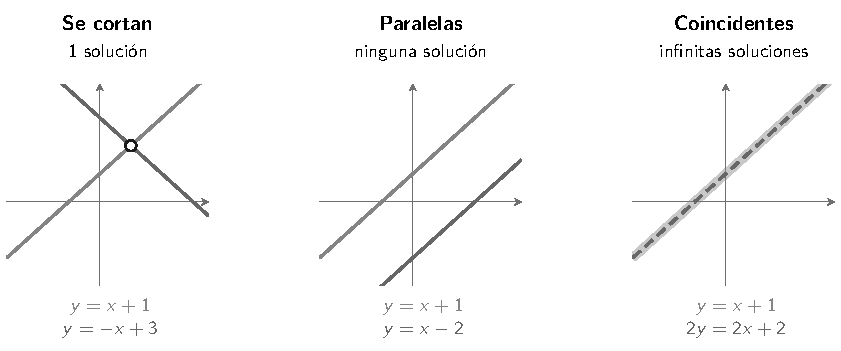
\includegraphics[width=0.85\linewidth]{sis_tres_casos}\end{center}
\begin{center}
\begin{tabular}{@{}llll@{}}
\toprule
Rectas & Despejando $y$ & Soluciones & Al resolver queda\\ \midrule
se cortan & distinta pendiente & una & $x$ e $y$\\
paralelas & misma pendiente, distinto corte & ninguna & algo falso, como $0 = -2$\\
coincidentes & todo igual & infinitas & $0 = 0$\\ \bottomrule
\end{tabular}
\end{center}
\begin{ejemplo} $x + 2y = 3$ y $x + 2y = 5$ son paralelas. $x + 2y = 3$ y $2x + 4y = 6$ son la misma recta: la segunda es la primera multiplicada por 2 en \textbf{todos} sus términos.\end{ejemplo}
\begin{ojo}[Nunca dos] Dos rectas distintas no se cortan en exactamente dos puntos.\end{ojo}

\begin{elejemplo}{Tipo PAES}
¿Cuál es la solución del siguiente sistema de ecuaciones?
\[ \begin{cases} 3x - 2y = 5 \\ x + 4y = 11 \end{cases} \]
\alts{$(2, 3)$}{$(1, -1)$}{$(3, 2)$}{$(7, 1)$}
\solucion{En la segunda la $x$ tiene coeficiente 1: sustitución. $x = 11 - 4y$, y en la primera, $3(11 - 4y) - 2y = 5$, o sea $33 - 14y = 5$, $-14y = -28$ e $y = 2$. Entonces $x = 11 - 8 = 3$. Comprobación: $9 - 4 = 5$ y $3 + 8 = 11$. $(2, 3)$ da vuelta el par, $(1, -1)$ solo cumple la primera y $(7, 1)$ solo la segunda.}{C}
\end{elejemplo}

%% =====================================================================
\section{Problemas con sistemas de ecuaciones}

\subsection{Del enunciado al sistema en 4 pasos}
\begin{clave}[Los 4 pasos] 1. Nombra las dos incógnitas, con su unidad. 2. Escribe una ecuación por cada dato total: casi siempre uno de \textbf{cantidades} y otro de \textbf{valor}. 3. Resuelve. 4. Responde y comprueba en el enunciado.\end{clave}
\begin{ejemplo}[Entradas] Adulto \peso 5000, niño \peso 3000; 80 entradas y \peso 300.000: $x + y = 80$ y $5000x + 3000y = 300.000$. Con $y = 80 - x$ se llega a $2000x = 60.000$: 30 de adulto y 50 de niño.\end{ejemplo}
\begin{ojo}[No mezcles] En la ecuación de cantidades no van precios, y en la de dinero cada cantidad va con \textbf{su} precio. $x + y = 300.000$ no tiene sentido: suma entradas y da pesos.\end{ojo}

\subsection{Monedas, edades y mezclas}
\begin{ejemplo}[Monedas] 30 monedas de \peso 100 y \peso 500 suman \peso 7400: $x + y = 30$ y $100x + 500y = 7400$. Dividiendo la segunda por 100, $x + 5y = 74$; restando la primera, $4y = 44$: 11 de 500 y 19 de 100.\end{ejemplo}
\begin{ejemplo}[Edades] Padre e hijo suman 50; hace 5 años el padre tenía 4 veces la edad del hijo: $p + h = 50$ y $p - 5 = 4(h - 5)$. Resulta $h = 13$ y $p = 37$.\end{ejemplo}
\begin{ojo}[Paréntesis en las edades] «4 veces la edad del hijo hace 5 años» es $4(h - 5)$, no $4h - 5$. Y el tiempo pasa para todos: en 4 años, $a + 4 = 3(h + 4)$.\end{ojo}
\begin{ejemplo}[Mezclas] Café de \peso 8000 y de \peso 12.000 el kilo para 20 kg a \peso 9000: $x + y = 20$ y $8000x + 12.000y = 20\cdot 9000$. Resulta 15 kg del barato y 5 kg del caro: el precio de la mezcla está más cerca del café barato.\end{ejemplo}
\gatotip[\gatolila]{Si el precio es «por kilogramo», la incógnita son \emph{kilogramos}, no frutas ni paquetes. La PAES pregunta justo eso.}

\subsection{Planes: ¿cuándo cuestan lo mismo?}
\begin{minipage}[c]{0.5\linewidth}
Plan A: \peso 8000 más \peso 50 por minuto; plan B: \peso 12.000 más \peso 30. Igualando, $8000 + 50m = 12.000 + 30m$: $m = 200$ minutos, con un costo de \peso 18.000 en ambos.

El punto donde se cortan las rectas es donde las dos cantidades valen lo mismo. Antes de 200 minutos conviene A; después, B.
\end{minipage}\hfill
\begin{minipage}[c]{0.46\linewidth}\centering
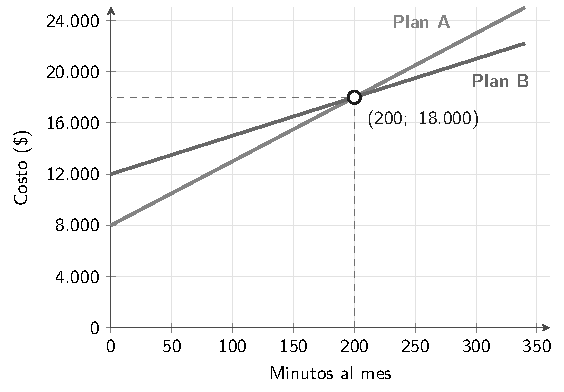
\includegraphics[width=\linewidth]{sis_planes}
\end{minipage}
\begin{ejemplo}[Tarifa fija] Con \peso 2300 por 40 minutos y \peso 3800 por 70: $f + 40v = 2300$ y $f + 70v = 3800$. Restando, $30v = 1500$: $v = 50$ y la tarifa fija es $f = 300$.\end{ejemplo}

\subsection{Qué representa cada parte del sistema}
En una obra de teatro la entrada de niño cuesta \peso 2000 y la de adulto \peso 3500; una familia pagó \peso 40.000 por 14 entradas:
\[ \begin{cases} x + y = 14 \\ 2000x + 3500y = 40.000 \end{cases} \]
\begin{clave}[Cantidad, precio o dinero] $x$ va con 2000: es la \textbf{cantidad} de entradas de niño. 2000 es un \textbf{precio}. $2000x$ es \textbf{dinero}: lo pagado por las entradas de niño. 40.000 es el total pagado y 14 el total de entradas.\end{clave}
\begin{ojo}[Porcentajes] Si aparece $\frac{80}{100}\cdot B$ como lo pagado con un 20~\% de descuento, $B$ es el precio \textbf{original}. Y no sumes lo que el enunciado excluye: «se recaudó solo por las poleras» deja fuera los envíos.\end{ojo}
\gatotip[\gatonegro]{Al final, relee qué representa cada letra: si piden las entradas de niño y respondes $y$, marcaste la otra.}

\begin{elejemplo}{PAES Invierno 2026, adaptada}
Una empresa dedicada a la venta de poleras ofrece a sus clientes dos opciones de diseño: personalizado o de catálogo. El precio por polera con diseño personalizado es \peso 8500 y con diseño de catálogo es \peso 7500. Adicionalmente, se hace un cobro por envío a domicilio de \peso 2500.

En un día de trabajo se vendió un total de 18 poleras en diez envíos y se recaudó \peso 146.000 solo por las poleras. Para calcular la cantidad de poleras con diseño personalizado que se vendieron, una persona realiza el siguiente procedimiento, cometiendo un error.

Paso 1: representa con $x$ la cantidad de poleras con diseño personalizado y con $y$ la cantidad de poleras con diseño de catálogo, y establece el sistema $\begin{cases} x + y = 18 \\ 8500x + 7500y = 146.000 + 25.000 \end{cases}$\\[2pt]
Paso 2: despeja $y$ de la primera ecuación, obteniendo $y = 18 - x$.\\
Paso 3: reemplaza $y$ en la segunda ecuación, obteniendo $8500x - 7500x = 146.000 + 25.000 - 7500\cdot 18$.\\
Paso 4: resuelve la igualdad anterior y determina que la cantidad de poleras con diseño personalizado es 36.

¿En cuál de los pasos la persona cometió el error?
\alts{En el Paso 1}{En el Paso 2}{En el Paso 3}{En el Paso 4}
\solucion{La primera ecuación está bien, pero en la segunda $8500x + 7500y$ es el dinero de las poleras, y el enunciado dice que se recaudaron 146.000 \textbf{solo por las poleras}: los $10\cdot 2500 = 25.000$ de los envíos no van ahí. El error está en el Paso 1. Los Pasos 2, 3 y 4 operan bien con lo que reciben. Lo correcto: $1000x = 146.000 - 135.000 = 11.000$, o sea 11 personalizadas y 7 de catálogo; $8500\cdot 11 + 7500\cdot 7 = 146.000$. Además, 36 poleras personalizadas es imposible si en total se vendieron 18.}{A}
\end{elejemplo}
